\chapter{Synthese mit reinen Tönen}


\begin{enumerate}[a)]
% a)
\item Siehe MATLAB-Code:
\begin{itemize}
\item
synthesize.m
\end{itemize}
\item
Siehe MATLAB-Code:
\begin{itemize}
\item
synthesize.m
\end{itemize}
\vspace{\baselineskip}
Um die zeitliche Hüllkurve zu realisieren, verwenden wir ein in zwei Hälften geteiltes Hann-Fenster, welches als Attack und Decay für einen reinen Sinuston fungiert. Der ansteigende Teil entspricht der Formel
\begin{align*}
w(n) &= 0.5 \cdot (1- \mathrm{cos}(2 \pi \frac{n}{N})) & n \in \left\{1,\,...\,,\,\frac{N}{2}\right\}
\end{align*}
und der abklingende Teil derselben Formel in einem anderen Wertebereich:
\begin{align*}
w(n) &= 0.5 \cdot (1- \mathrm{cos}(2 \pi \frac{n}{N})) & n \in \left\{\frac{N}{2}+1,\,...\,,\,N\right\}
\end{align*}
Die Form der Einschwing- und Anklingkurve ist in Abbildung \ref{fig:env} zu sehen.
\begin{figure}[h!]
  \centering
      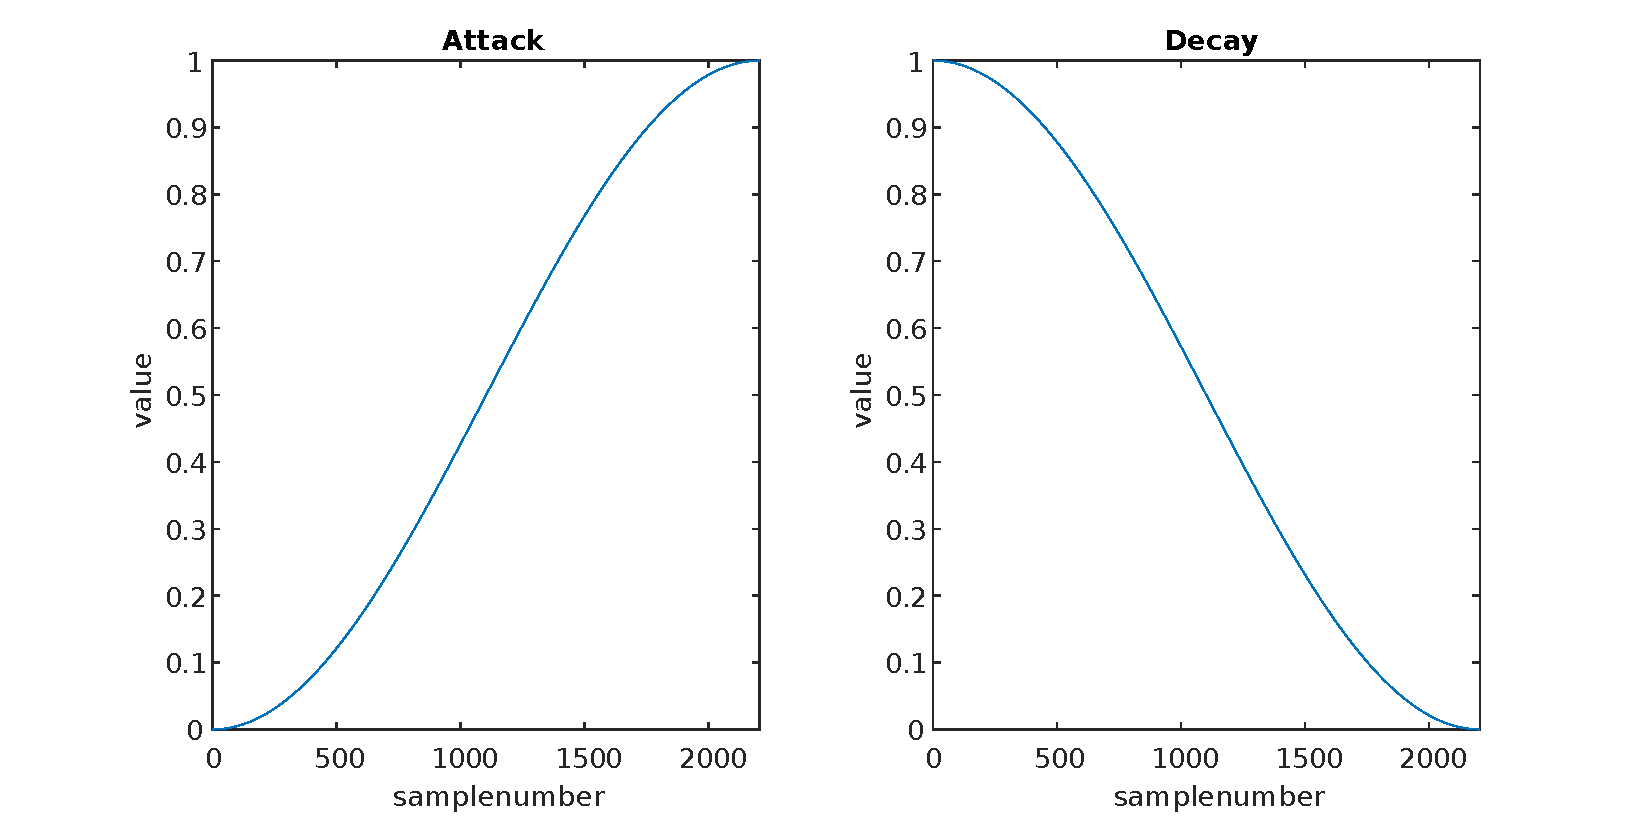
\includegraphics[width=\textwidth]{Figures/envelopeplot}
 \caption{In zwei Hälften geteiltes Hann-Fenster für die zeitlichen Attack- und Decay-Hüllkurven der Sinustöne. Länge: t = 0.05 s bei fs = 44100 Hz}
	\label{fig:env}
\end{figure}
\item
Die Unterschiede zwischen gleichstufiger und pythagoräischer Stimmung sind hörbar. Die pythagoräischen Versionen beider Stücke klingen im Gegensatz zur gewohnten gleichstufigen Stimmung mal mehr mal weniger verstimmt, je nachdem welche Intervalle gespielt werden. Es ist für uns schwer zu beschreiben, an welchen Stellen der Effekt besonders stark zum Tragen kommt. Beim Blick auf Abbildung \ref{fig:f1} wir klar, dass beim Stück in C-Dur der Unterschied z.B. bei den großen Terzen von C zu E deutlicher hörbar sein sollte, als bei einer Quinte von C zu G. \\
Das Stück in Ges-Dur klingt im pythagoräischen System noch etwas schiefer, als das in C-Dur. Hier ist z.B. die Quinte zwischen Ges und Des besonders stark betroffen.\\ 
\end{enumerate}
